\section{Experimental Setup}
\label{sec:setup}

\subsection{Simulation Environment and Software Stack}
\label{sec:setup-stack}
Experiments run on ROS~2 Humble with Gazebo Fortress (Ignition Gazebo~6) as the
physics simulator, bridged through \texttt{ros\_gz}. The robot is a
differential-drive platform (\emph{inspector\_bot}) with a 360$^\circ$ planar
range sensor. Global path planning uses the Nav2 stack with the
\emph{NavfnPlanner} global planner and a Model Predictive Path Integral (MPPI)
controller for path following (differential motion model, control frequency
$20$~Hz) over a \emph{static} occupancy map. The Nav2 stack is configured with
Adaptive Monte Carlo Localization (AMCL), but in these experiments the
map$\rightarrow$odom transform is held fixed so that the robot pose is exact and
localization drift is not modeled (its treatment is left as future work,
Section~\ref{sec:setup-repro}); the pose used by the perception and metrics nodes
is therefore the ground-truth map-frame transform, not an AMCL estimate. The
costmaps use a robot radius of $0.25$~m, an
inflation radius of $0.55$~m and a cost-scaling factor of $3.0$; the goal
tolerance is $0.25$~m.

The world models a simplified substation (Fig.~\ref{fig:world}): a power
transformer ($3{\times}2{\times}1.5$~m at $(10,10)$), a circuit breaker
($1{\times}1{\times}2$~m at $(-5,5)$), a busbar ($8{\times}0.3{\times}0.3$~m at
$(0,15)$) and a $50{\times}50$~m perimeter fence, on a ground plane. The static
occupancy map ($1040{\times}1040$ cells at $0.05$~m/cell) is aligned with the
world frame, so waypoints in world coordinates serve directly as navigation
goals. The deliberative patrol visits five waypoints
(in metres): $(13,-8)$, $(13,10)$, $(0,11)$, $(-8,5)$ and a return at
$(-10,-10)$.

\begin{figure}[t]
\centering
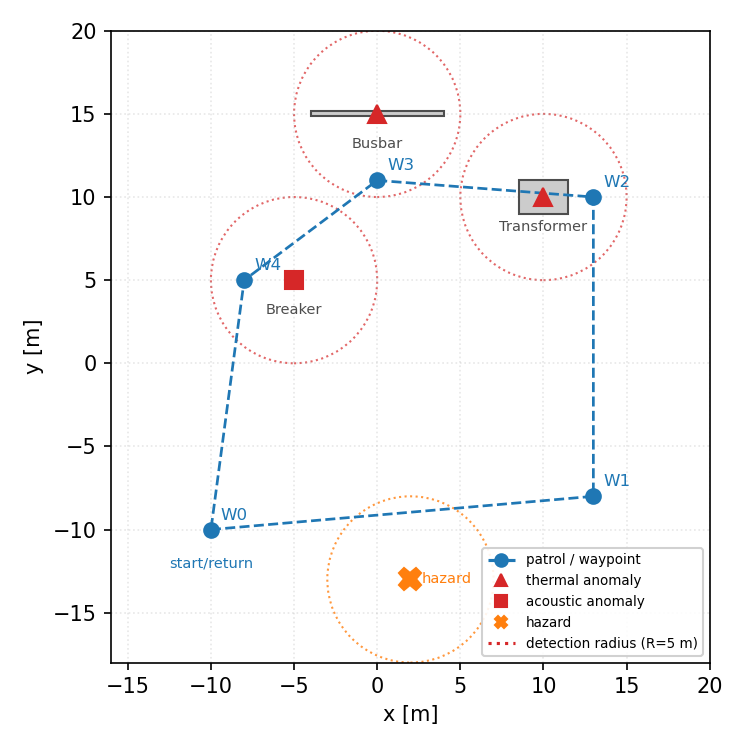
\includegraphics[width=\columnwidth]{world_map}
\caption{Substation scenario (default): equipment (gray), the five patrol
waypoints W0--W4 and the round (dashed), the attraction anomalies (thermal
$\triangle$, acoustic $\square$) and the hazard ($\times$), each with its
$R=5$~m detection radius (dotted). Coordinates in metres, world frame.}
\label{fig:world}
\end{figure}

\subsection{Simulated Events}
\label{sec:setup-events}
Following Section~\ref{sec:method-sensing}, the perception output is abstracted
as events. The \emph{default} scenario has three attraction anomalies --- a
thermal event at the transformer $(10,10)$, a thermal event at the busbar
$(0,15)$ and an acoustic event at the breaker $(-5,5)$ --- and one persistent
hazard (repulsion) beside the first patrol leg at $(2,-13)$. The \emph{adverse}
scenario (E5) densifies the anomalies into clusters (five anomalies: two near
the transformer and two near the breaker, plus the busbar), so that multiple
events fall within the sensory radius simultaneously and the layer must
arbitrate between them; the hazard is unchanged. The \emph{route-hazard} scenario
(RHM/RHB) keeps the three default anomalies but moves the hazard \emph{onto} the
first patrol leg at $(1.5,-9)$---directly blocking the path to the next
waypoint---so that a purely reactive retreat cannot resolve it without deviating
the route; here the detected hazard is also projected, at its \emph{perceived}
position, as a \emph{persistent} keepout into the global costmap (a mark the
deliberative planner routes around for the rest of the mission). The \emph{conflict} scenario
(CONF) keeps the three default anomalies and co-locates, at the default hazard's
position $(2,-13)$, a \emph{strong} acoustic anomaly ($I_e=0.95$,
$|w\,I_e|=1.14$) with a \emph{weaker} hazard ($I_e=0.70$, $|w\,I_e|=1.05$): the
attraction is the more salient of the two, so a magnitude-only rule would prefer
inspection, whereas the precedence rule must trigger \textsc{Avoid}. The
detection radius is $R=5$~m, the inspection standoff $\rho=2$~m and the retreat
margin $\Delta=1.5$~m (full coordinates and intensities in
Appendix~\ref{app:params}).

\subsection{Experimental Matrix and Metrics}
\label{sec:setup-matrix}
We evaluate the affective layer against a fixed baseline and an
artificial-potential-field baseline, across an $\eta$ sweep, an $\eta=0$ (affective-value) ablation,
an adverse scenario, a hazard placed on the route, and perception-noise
perturbations (Table~\ref{tab:matrix}); each configuration is run $n=10$ times
(headless, $600$~s timeout per run). \textbf{E1} is the deliberative patrol
\emph{without} the reactive layer (no affective response). \textbf{E0} is an
ablation that enables \textsc{Stay Alert} but sets the value-update weight
$\eta=0$. \textbf{E2--E4} enable the full method with
$\eta\in\{0.3,0.5,0.8\}$, and \textbf{E5} uses $\eta=0.5$ on the adverse
scenario. \textbf{APF} replaces the reactive layer with a conventional
artificial-potential-field controller acting on the same events. \textbf{RHM}
and \textbf{RHB} place the hazard \emph{on} a patrol leg---for the method (with
the detected hazard projected as a persistent deliberative keepout) and for
the fixed baseline, respectively. \textbf{N1} and \textbf{N2} repeat the method
under moderate and high zero-mean Gaussian perception noise on event position and
intensity. \textbf{CONF} co-locates a strong attraction event with a weaker
hazard (Section~\ref{sec:setup-events}) to test whether the safety precedence of
Eq.~\eqref{eq:phi-update} holds when both event types are simultaneously within
range. \textbf{KOa} and \textbf{KOb} ablate the on-route safety response into its
two mechanisms---keepout only (reactive retreat disabled) and retreat only
(deliberative keepout disabled)---so that RHM (both), KOa, and KOb isolate the
contribution of each to passing an on-route hazard. \textbf{DHa} and \textbf{DHb}
run a \emph{directed} test of the reactive retreat's transient value: in the
\emph{dyn-hazard} scenario a hazard is co-located with an anomaly and stays
\emph{inactive} until the robot---already committed to inspecting it---closes to
$3$~m, at which point it activates (the environment decides when the hazard
appears). DHa enables the reactive retreat (with keepout) and DHb disables it
(keepout only), isolating what the retreat adds when a hazard \emph{emerges during}
an investigation, a case the static scenarios cannot exercise. The method and
simulation hyperparameters are summarized in Table~\ref{tab:hyper}.

\begin{table}[t]
\centering
\caption{Experimental matrix ($10$ attempted runs each).}
\label{tab:matrix}
\begin{tabular}{llccc}
\hline
\textbf{Exp.} & \textbf{Reactive layer} & $\bm{\eta}$ & \textbf{Scenario} &
\textbf{\#anom./haz.}\\
\hline
E1  & none                 & --   & default      & 3 / 1\\
E0  & Stay Alert (ablation)& 0    & default      & 3 / 1\\
E2  & Stay Alert           & 0.3  & default      & 3 / 1\\
E3  & Stay Alert           & 0.5  & default      & 3 / 1\\
E4  & Stay Alert           & 0.8  & default      & 3 / 1\\
E5  & Stay Alert           & 0.5  & adverse      & 5 / 1\\
APF & potential field      & --   & default      & 3 / 1\\
RHM & Stay Alert           & 0.5  & route-hazard & 3 / 1\\
RHB & none                 & --   & route-hazard & 3 / 1\\
N1  & Stay Alert (noise m.)& 0.5  & default      & 3 / 1\\
N2  & Stay Alert (noise h.)& 0.5  & default      & 3 / 1\\
CONF& Stay Alert           & 0.5  & conflict     & 4 / 1\\
KOa & keepout only         & 0.5  & route-hazard & 3 / 1\\
KOb & retreat only         & 0.5  & route-hazard & 3 / 1\\
DHa & retreat $+$ keepout  & 0.5  & dyn-hazard   & 1 / 1\\
DHb & keepout only         & 0.5  & dyn-hazard   & 1 / 1\\
\hline
\end{tabular}
\end{table}

Each run is logged by a metrics node and reduced to its final values. We report:
\emph{anomalies inspected} (unique, credited only when the reactive navigation
\emph{succeeds}, a commanded dwell of $t_{\text{dwell}}$ elapses, and the simulator
confirms the robot's final pose lies within a \emph{confirmation distance} of the
\emph{true} target---the standoff plus a tolerance, $\rho + 1.3 = 3.3$~m; the dwell
is enforced by the controller rather than independently verified, so this metric
measures \emph{confirmed arrival within $3.3$~m plus a commanded dwell}, a proxy for
physical inspection, not the full standoff-and-orientation condition);
\emph{investigation time}; \emph{route deviations} (affective triggers);
\emph{hazard avoidances} (retreat events); \emph{minimum hazard distance}
(closest approach to a hazard, higher is better); and, for the on-route hazard,
safety-oriented \emph{proxies} computed from the true hazard position:
\emph{contact-region entries} (``collisions''; centre-to-centre distance below
$0.5$~m, a simulated proxy rather than a physical contact sensor), \emph{time below
a clearance threshold} ($2$~m, centre-to-centre), \emph{minimum radial
time-to-collision}
($d/\dot d$ to the nearest hazard, an approaching-rate proxy, not a
trajectory-intersection time), and \emph{retreat success}; \emph{mission duration};
\emph{distance travelled}; and the complete value-update residual
$|\alpha\delta+\eta\Phi|$ as a stability proxy. Because several outcomes are
bounded counts with (near-)zero variance, group comparisons use distribution-free
%% Nomenclatura dos instrumentos geometricos: ambos sao ENTRADAS EM REGIAO
%% definida operacionalmente por distancia, nao contato fisico nem distancia
%% regulamentar. Sem a calibracao pelo raio do robo o leitor nao consegue julgar o
%% que 0.5 m significa.
Both geometric safety instruments are entries into regions defined operationally by
centre-to-centre distance, counted on the rising edge, and computed against the
\emph{true} hazard position with the robot pose taken from the \texttt{map} frame.
Neither is a physical contact measurement, and neither is a regulatory electrical
clearance. To let the reader calibrate them: the robot radius configured in the
planner is $0.25$~m, so the $0.5$~m contact region corresponds to the robot body
reaching the hazard centre, and the $2$~m band to $1.75$~m of clearance from the
robot's edge. The $2$~m value is a diagnostic threshold adopted for measuring
exposure in this evaluation; the study declares no minimum-clearance requirement, so
transiting below it is not a requirement violation but an exposure that we report.

tests (Mann--Whitney $U$, exact for untied samples with $n_1+n_2\le20$ and by
permutation for degenerate arms; see Section~\ref{sec:results}) with the Cliff's
$\delta$ effect size, $95\%$ bootstrap confidence intervals, numeric $p$-values,
and Holm correction across the confirmatory family; equivalence claims use a two
one-sided test (TOST) against a pre-declared margin, and per-mission success rates
use Wilson-score intervals. Runs in which the platform failed to initialize are
excluded as a startup-reliability outcome.

\begin{table}[t]
\centering
\caption{Method and simulation hyperparameters.}
\label{tab:hyper}
\begin{tabular}{lll}
\hline
\textbf{Group} & \textbf{Parameter} & \textbf{Value}\\
\hline
Value update & learning rate $\alpha$ & 0.1\\
(App.~\ref{app:update}) & discount $\gamma$ & 0.95\\
          & affective weight $\eta$ & 0.3 / 0.5 / 0.8\\
          & cell size $\delta$; buckets $B$ & 1.0~m; 4\\
          & progress reward $r_{\text{prog}}$ & 1.0\\
Field $\Phi$ & weights (therm./acou./haz.) & 1.0 / 1.2 / $-1.5$\\
          & thresholds $\theta_m$ & 0.4 / 0.3 / 0.3\\
          & decay $\lambda$; clip $\Phi_{\max}$ & 0.85; 2.0\\
          & decay period $T_d$; residual $\varepsilon$ & 1~s; $10^{-3}$\\
\textsc{Stay Alert} & enter $\theta_{\text{in}}$; exit $\theta_{\text{out}}$ & 0.45; 0.25\\
          & dwell $t_{\text{dwell}}$; budget $t_{\max}$ & 3~s; 40~s\\
          & refractory $t_{\text{ref}}$ & 8~s\\
Evaluator & confirm.\ distance (metric) & 3.3~m\\
Keepout   & project radius; disc radius & 5~m; 1.2~m\\
APF base. & standoff; budget & 1.8~m; 30~s\\
Events    & radius $R$; standoff $\rho$ & 5~m; 2~m\\
          & retreat margin $\Delta$ & 1.5~m\\
\hline
\end{tabular}
\end{table}

\subsection{Reproducibility}
\label{sec:setup-repro}
The full code, world, launch files, the batch runner and the analysis script
are publicly available\footnote{\texttt{github.com/voidmmn/tese\_react\_nav}}.
Installation scripts set up ROS~2
Humble, Gazebo Fortress and Nav2; a batch script runs the full matrix
and writes one CSV per run, and the analysis script produces the summary table,
the effect-size and distribution-free comparisons, and the boxplots (the boxplot
and value-residual figures are produced by released scripts). Alongside the
per-run CSVs of aggregate counts, we release a \emph{consolidated per-episode
audit trail} (\texttt{audit\_trail.csv}), regenerated by a released script from the
per-episode log messages of both the evaluator and the supervisor. Each row is
keyed by configuration, run seed and episode, and carries: for an investigation,
the target identity and its \emph{true} position, and the outcome---the confirmed
arrival distance (\emph{inspected}), a confirmation \emph{rejected} with its
distance and threshold, an \emph{inspection\_failed} with its cause
(timeout / navigation), or \emph{deferred}; for the reactive avoid, its entry, its
exit reason (\emph{safe} / \emph{retreated} / \emph{timeout}), and the reactive
navigation goal's \emph{nav\_result} (aborted / cancelled / rejected); and, for the
dynamic-hazard scenario, the hazard-activation instant (in simulation time) and the
first keepout and reactive publications with the robot pose. The schema keeps the
target's true position and the robot's pose in \emph{separate} columns and records
both the simulation time (where the message carries it) and the log timestamp.
From this trail the confirmation rejections, the inspection failures, and the avoid
outcomes reported throughout Section~\ref{sec:results} (the dynamic-hazard,
adverse and perception-noise analyses) are auditable per episode; its
investigation, credit, deferral and \textsc{Stay Alert} avoid counts cross-check
the corresponding aggregate CSVs. The avoid-event extraction covers the
\textsc{Stay Alert} supervisor; the APF baseline logs its avoidances through a
different path, so those events are counted in the aggregate CSVs but not itemized
in the trail. Experiments
ran on a workstation (Intel Xeon W-1350, 12~cores, 16~GB RAM) under Ubuntu~22.04
(WSL2), headless, at a near real-time factor ($\mathrm{RTF}\approx1$); the
perception-noise generator is seeded \emph{per repetition} (the run index is passed
as the seed and recorded in each CSV), while the remaining run-to-run variation is
the inherent stochasticity of the physics simulator and of the timing in the
navigation stack. The exact code version that produced the
reported results is archived under the tagged release
\texttt{v1.0-resubmission} in the repository. Three configurations---the dense
scenario E5 and the two dynamic-hazard trials DHa and DHb---were re-run under the
corrected hazard-activation and failure-handling code; the other thirteen were
reused. This reuse is a \emph{verifiable identity}, not an assumption: those
thirteen record zero navigation aborts, cancellations, and rejections, so the
corrected failure-handling path is never exercised in them and their metrics are
unchanged under either version, as their published counters show. A provenance
manifest (\texttt{PROVENANCE.md}) records the reference snapshot for each batch, the
per-run seeds, and SHA-256 checksums of all $160$ CSVs, and identifies the replaced
files; the mobile tag alone does not fix this correspondence. As the contribution is the affective
navigation policy operating on abstracted events, it does not depend on raw range
data: obstacle geometry is provided by the static map, and the odometry is kept
exact (the map$\rightarrow$odom transform is held fixed), so we do \emph{not}
model localization drift here; robustness to localization error, event
persistence, and map geometry is left as future work, complementing the
perception-noise sweep of Section~\ref{sec:robustness}.
